

\section{Particle Physics and the Standard Model}

Particle physics studies the elementary building blocks of matter, radiation and the interactions between them. So far, there are six quarks, six leptons, four gauge bosons types, and one Higgs boson within the family of elementary particles, whose dynamics are governed by symmetries and conservation laws. Elementary particles help to build the rich structure of nuclei, atoms, and macroscopic matter. Similarly, the forces between particles arise from the exchange of gauge bosons and are associated with the local symmetries \cite{griffiths_book}.


%\begin{figure}[tbh]
\begin{figure}[H]
  \centering
  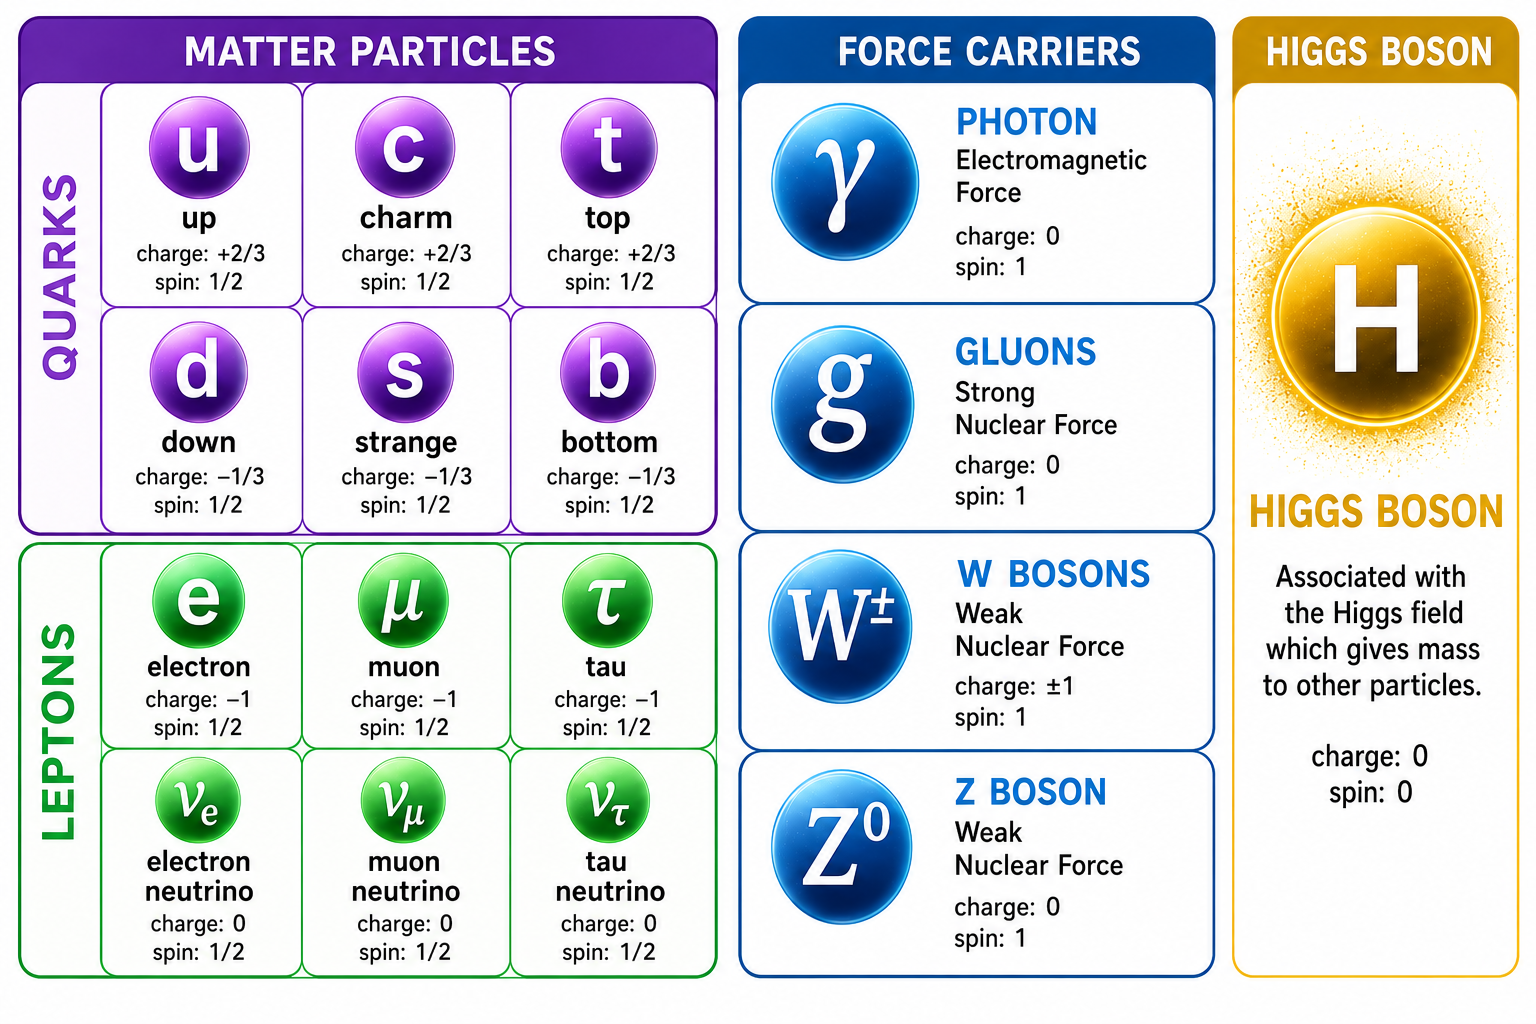
\includegraphics[width=0.8\textwidth,
    alt={Chart of the Standard Model particles with their charge and spin:
         six quarks (up, down, charm, strange, top, bottom), six leptons
         (electron, muon, tau and their neutrinos), the force carriers
         (photon, gluon, W and Z bosons) and the Higgs boson.}]{Images/123_Plots/StandardModel.png}
  
  \caption{A schematic overview of the Standard Model showing fundamental particles and force carriers. This image was generated with the help of ChatGPT.}
  
  \label{fig:standard_model}
  
\end{figure}


The ``Standard Model'' organizes the elementary particles into three categories: matter \textbf{fermions}, \textbf{gauge bosons}, and the \textbf{Higgs boson}. As a reference from figure \ref{fig:standard_model}, quarks and leptons makes fermions, while all the force carrier makes gauge bosons. There are six different flavors (like u, d, s, c, b, t) of quarks and all of them carry color charge, and participate in strong, weak and electromagnetic interaction. The leptons \((e, \mu, \tau\)) and their corresponding neutrinos are colorless and do not interact via strong force \cite{halzen_quarksleptons, griffiths_book}.


\section{Quantum Chromodynamics (QCD)}
 
Quantum Chromodynamics (QCD) is the theory of the strong interaction in the Standard Model. It describes the behavior of quarks and gluons through the exchange of color charge \cite{peskin_QFT, griffiths_book}. \ac{QCD} is a non-Abelian gauge theory built on the \(SU(3)_C\) color symmetry group, where gluons not only mediate force between quarks but also interact among themselves \cite{peskin_QFT}.

\subsection{QCD Lagrangian}

The dynamics of quarks and gluons are encoded in the \ac{QCD} Lagrangian density, which for \(N_f\) quark flavors can be written as \cite{lancaster2014qft, ellis1996qcd, peskin_QFT}

\begin{equation}
\mathcal{L}_{\text{QCD}} = \sum_{f=1}^{N_f} \bar{\psi}_f \left( i \gamma^\mu D_\mu - m_f \right) \psi_f - \frac{1}{4} F_{\mu\nu}^a F^{\mu\nu}_a
\label{eq:QCD_lagrangian}
\end{equation}

where \(\psi_f\) denotes the quark field of flavor \(f\), \(m_f\) is the corresponding quark mass, and \(D_\mu\) is the covariant derivative that couples quarks to the gluon gauge fields. The gluon field strength tensor \(F_{\mu\nu}^a\) describes both the propagation of gluon fields and their self-interactions, reflecting the non-Abelian nature of the \(SU(3)_c\) gauge symmetry \cite{lancaster2014qft, ellis1996qcd, peskin_QFT}.




\subsection{The Running Coupling Constant}

The strong coupling constant ($\alpha_s$) is the fundamental parameter governing the strength of the strong interaction in Quantum Chromodynamics. Analogous to the electromagnetic fine structure constant ``$\alpha_{\mathrm{em}} = e^2/(4\pi)$'', it is defined in terms of the \ac{QCD} gauge coupling ``$g_s$'' as \cite{deur2016qcd}

\begin{equation}
\alpha_s(\mu^2) \equiv \frac{g_s^2(\mu^2)}{4\pi},
\label{eq:coupling_const_QCD}
\end{equation}
where $\mu$ denotes the renormalization scale.


The equation \ref{eq:coupling_const_QCD}, being an example of non Abelian theory, have the scale dependence feature. This means ``$\alpha_s$'' in equation \ref{eq:coupling_const_QCD} cannot be determined exactly and must be approximated separately in different energy scale. When $Q^2 > \Lambda_{\mathrm{QCD}}^2$, we use perturbation expansion and the equation \ref{eq:coupling_const_QCD} takes the following form \cite{deur2016qcd}:

\begin{equation}
\alpha_s(\mu^2)
=
\frac{4\pi}{\beta_0 \ln\!\left(\mu^2/\Lambda_{\mathrm{QCD}}^2\right)},
\label{eq:coupling_const_pQCD}
\end{equation}

where $\Lambda_{\mathrm{QCD}}$ is the \ac{QCD} scale parameter. In applications to physical processes characterized by a momentum scale $Q$, it is common to choose the renormalization scale $\mu^2 = Q^2$, so that the coupling is written as $\alpha_s(Q^2)$. In the regime where $Q^2 \gg \Lambda_{\mathrm{QCD}}^2$, the logarithm in the denominator of the equation \ref{eq:coupling_const_pQCD} becomes large enough to make the coupling constant parametrically small, ($\alpha_s(Q^2) \ll 1$). Therefore, at much higher $Q^2$ region (high energy or short distance), \ac{QCD} interactions become weak and develops the property of asymptotic freedom.


